\documentclass[11pt, oneside]{article}   	% use "amsart" instead of "article" for AMSLaTeX format
\usepackage{geometry}                		% See geometry.pdf to learn the layout options. There are lots.
\geometry{letterpaper}                   		% ... or a4paper or a5paper or ... 
%\geometry{landscape}                		% Activate for for rotated page geometry
%\usepackage[parfill]{parskip}    		% Activate to begin paragraphs with an empty line rather than an indent
\usepackage{graphicx}				% Use pdf, png, jpg, or eps§ with pdflatex; use eps in DVI mode
								% TeX will automatically convert eps --> pdf in pdflatex		
\usepackage{amssymb}
\usepackage{amsmath}
\usepackage{parskip}
\usepackage{color}
\usepackage{hyperref}

\title{Integrating functions of a complex variable}
%\author{The Author}
%\section{}
%\subsection*{}
\date{}							% Activate to display a given date or no date

\graphicspath{{/Users/telliott_admin/Dropbox/Tex/png/}}
% \begin{center} 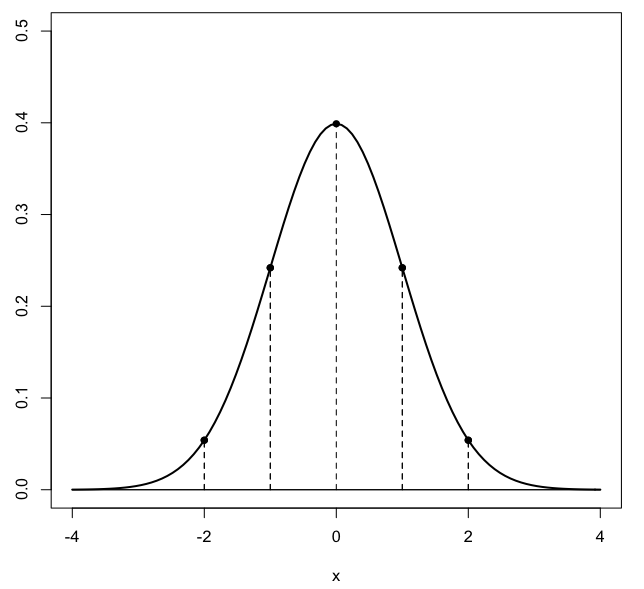
\includegraphics [scale=0.4] {gauss3.png} \end{center}
\begin{document}
\maketitle
\Large
Complex functions are differentiated and integrated in a way that is similar to real functions, with these differences:  normally, we restrict our attention to functions that are analytic, and we pay attention to points in the complex plane where they have poles (or singularities).  

Also, the integrals that we compute are line integrals.

In general terms, a complex function is a function that produces a complex number as the result.  And the most general case is that the input is a complex number as well.  Se we could write:
\[ w = f(z) \]
where both $w$ and $z$ are complex numbers.

In this case we can look at the parts of $f$ that generate the real and imaginary parts of $w$ as separate functions:
\[ w = f(z) \]
\[ = u(x,y) + iv(x,y) \]

However, things may be simpler and often are.  The reason is that $x$ and $y$ may be related because we are following a curve in the complex plane.  We'll see why later.  For now, following a curve means that $u$ and $v$ are both parametric equations of a parameter $t$ and that parameter is \emph{real}.

So a lot of the proof relating to this stuff follow directly from calculus.

\subsection*{getting started}

\[ z = x + i y \]
\[ dz = dx + i dy \]
and the function
\[ w = f(z) \]
\[ = u(x,y) + iv(x,y) \]
we can write as
 \[ \int f(z) \ dz = \int (u + i v) (dx + i dy) \]
\[ = \int (u + iv) \ dx + (- v + i u) \ dy \]
\[ = \int u \ dx - v \ dy + iv \ dx + iu \ dy \]

The integral of a complex function is defined as a sum of integrals of two real variables.  Just as with line integrals for real functions of $x$ and $y$, the variables are related by the curve over which we will integrate.

Recall that for the work integral
\[ \int_C \mathbf{F} \cdot d \mathbf{r} = \int_C M \ dx + N \ dy \]
we parametrize the curve to get the integral over a single variable.

We can view $y$ as a function of $x$ or perhaps, we can parametrize both $x$ and $y$ as functions of $t$.

Suppose our function is simply $z = x + iy$.  The integral is 
\[ \int z \ dz = \int (x + iy) (dx + i dy) \]
\[ = \int x \ dx - y \ dy + i x \ dy + i y \ dx \]

Now we must get $y$ in terms of $x$ from the curve.  Suppose the curve goes from $(1,i)$ to $(3,i)$, then to $(3,3i)$ and finally back to where we started.  

We have three segments.  Along the first part, we are moving in the positive $x$ direction, with no change in $y$, so $dy=0$ and $y = 1$, a constant, and the integral is
\[ \int x \ dx - y \ dy + i x \ dy + i y \ dx \]
\[ = \int x \ dx + i y \ dx \]
\[ = \int_{x=1}^{x=3} \ x + i  \ dx \]
\[ = \frac{x^2}{2} + ix \ \bigg |_1^3 \]
\[ = 4 + 2i \]

Along the second part, we are moving in the positive $y$ direction with $dx = 0$ and $x = 3$ so
\[ \int x \ dx - y \ dy + i x \ dy + i y \ dx \]
\[ = \int_{y=1}^{y=3} - y \ dy + 3 i \ dy \]
\[ = -\frac{y^2}{2} + 3iy \ \bigg |_1^3 \]
\[ = -4 + 6i \]

And for the third, both $dx$ and $dy$ are non-zero, so we must actually do the parametrization.  The curve is $y=x$.  Hence $dy = dx$.
\[ \int x \ dx - y \ dy + i x \ dy + i y \ dx \]
\[ = \int x \ dx - x \ dx + i x \ dx + i x \ dx \]
\[ = 2i \int x \ dx \]
Consider first the direction of the path as going from $(1,1)$ to $(3,3)$.
\[ = 2i \int_{x=1}^{x=3} x \ dx \]
\[ = 2i \ \frac{x^2}{2} \ \bigg |_1^3 \]
\[ = 2i \ \frac{8}{2} = 8i \]
However, for the closed path, where we end up back at the starting point, $C3$ should be moving from $(3,3)$ to $(1,1)$ so we have 
\[ 2i \ \frac{x^2}{2} \ \bigg |_3^1 = 2i \ - \frac{8}{2} = -8i \]
Notice that 
\[ \int_{C1} + \int_{C2} = 8i  = - \int_{C3}\]
If we follow the curve $C3$ from $(3,3)$ to $(1,1)$, the whole thing is just zero.  Later we'll see that this is not a coincidence.

\subsection*{example}
Suppose the function is
\[ f(z) = y - x - i3x^2 \]
and we proceed from the origin to the point $z = 1 + i$ either directly ($C_2$) or by first going up vertically and then across ($C_1$).

For the vertical part of $C_1$ we have that $x = 0$ and $dx = 0$.
\[ I = \int ( y - x - i3x^2 )\ (dx + idy) \]
\[ = \int y i \ dy \]
It's important to recognize that although we are proceeding from the point $z=0$ to the point $z = i$, the upper bound on this integral is not $i$ but $y = 1$!  Hence
\[ I = i\frac{y^2}{2} \ \bigg |_0^1 = \frac{i}{2} \]
For the horizontal part of $C_1$ we have that $y=1$ and $dy = 0$ so
\[ I = \int ( y - x - i3x^2 )\ (dx + idy) \]
\[ = \int (1 - x - i3x^2) \ dx \]
\[ = x - \frac{x^2}{2} - ix^3 \ \bigg |_0^1 = \frac{1}{2} - i \]
Therefore the total
\[ I = \frac{i}{2} + \frac{1}{2} - i = \frac{1}{2} \ (1 - i) \]
When going directly from the origin to $1 + i$ we relate $x$ to $y$ by the equation of the line $y=x$ so $dy = dx$ and
\[ I = \int ( y - x - i3x^2 )\ (dx + idy) \]
\[ = \int - i3x^2 \ (dx + i dx) \]
\[ = -i  \ x^3 \ \bigg |_0^1 + x^3 \ \bigg |_0^1 = -i \cdot 1 + 1 = 1  - i \]
And around the closed curve going backward along $C_2$:
\[ \oint f(z) \ dz =  \frac{1}{2} \ (1 - i) - (1  - i ) = -\frac{1}{2} (1 + i) \]

\end{document}  